\chapter{Pipeline Design and Execution}

The \gls{ngs}-pipeline represents a comprehensive solution for \gls{ngs} data analysis, designed to streamline the process of \gls{trimming}, \gls{genome} Assembly, and \gls{assembly} Quality Assessment. By integrating advanced bioinformatics tools such as fastp for \gls{trimming}, SPAdes for \gls{assembly}, and QUAST for Quality Evaluation, this pipeline ensures high fidelity in data processing and analysis. The entire codebase of the \gls{ngs}-pipeline is openly accessible at \url{https://github.com/shliamin/NGS-pipeline/blob/main/main.nf}, facilitating its adoption and customization for diverse research needs.

\section{Data Foundation}

\subsection{Input Data}
The data for the analysis were sourced from the publicly available Sequence \gls{read} Archive (SRA) at the National Center for Biotechnology Information (NCBI). Due to technical constraints and to ensure compatibility with the computing environment, it was decided to directly install SRA-Tools for command-line usage.

The procedure for downloading SRA-formatted data involved the use of the \texttt{prefetch} command, followed by conversion to \gls{fastq} using \texttt{fasterq-dump}, with the \texttt{--split-3} option employed for processing Paired-End \gls{read}s. For instance, to obtain data for Paired Genomic \gls{dna} Sequencing Analysis, the following commands were executed:
\begin{verbatim}
./prefetch SRR26630744
./fasterq-dump --split-3 SRR26630744
\end{verbatim}

This process successfully produced the necessary files for the analysis of paired genomic \gls{sequencing}: \texttt{SRR26630744\_1.fastq} and \texttt{SRR26630744\_2.fastq}. This approach requires \gls{read}s from both ends of a \gls{dna} fragment, a technique referred to as \gls{paired-end}. Typically, \gls{paired-end} involves two files, each containing \gls{read}s from one end of the fragment. This data was then consistently used for each run of the software pipeline and testing of different methods of \gls{trimming}, thus producing consistent results within the scientific method of research.


\subsection{Data Preprocessing}

Data preprocessing is a critical step in the pipeline, aimed at improving the quality of the input data for subsequent analyses. The preprocessing includes Quality \gls{trimming}, Sliding Window \gls{trimming}, Adapter Removal, Length Filtering, and Complexity Filtering as well as their hybrids with different parameters. These steps are executed using fastp, chosen for its versatility and high performance. The process not only reduces the computational load by removing low-quality sequences but also enhances the reliability of \gls{genome} Assemblies by reducing the number of regions of the \gls{genome} whose sequence is unknown or uncertain in a given context.



\section{Software Utilized}

This section details the computational tools and software (\autoref{table:software}) utilized in the pipeline. Each tool was selected based on its efficiency, accuracy, and compatibility with the overall design of the pipeline. The versions of the software are specified to ensure reproducibility and consistency of the analysis. The following table summarizes the software tools and their respective versions used:

\begin{table}[ht]
\centering
\begin{tabular}{l l}
\hline
\textbf{Software} & \textbf{Version} \\ \hline
Nextflow & 23.10.0 \\
fastp & 0.23.4 \\
SPAdes & 3.15.5 \\
QUAST & 5.2.0 \\ \hline
\end{tabular}
\caption{Summary of software tools and versions used in the pipeline.}
\label{table:software}
\end{table}

\subsection{fastp for Trimming}

\textit{fastp} is utilized within our pipeline for its efficiency in \gls{trimming} low-quality bases and removing adapters from raw sequencing reads. The tool's versatility allows for the execution of a variety of \gls{trimming} Combinations, enhancing the quality of data for downstream analysis. The \gls{trimming} combinations implemented are described below:

\paragraph{\gls{trimming} Combinations:}
The \gls{trimming} Combinations, such as \textit{QualityTrim\_Q25} and \textit{AdapterTrim\_Q25}, employ a systematic approach that combines the \gls{trimming} Type with specific parameters, delineated by underscores (\_). Initially, five basic \gls{trimming} Methods (\autoref{table:basic_trimming_methods}) with averaged parameters are applied, addressing various potential issues in sequencing data:

\begin{itemize}
    \item \textbf{Quality Trimming:} Removes regions with low sequencing quality to improve downstream analysis accuracy.
    \item \textbf{Adapter Trimming:} Excises adapter sequences to prevent interference in read alignment and analysis.
    \item \textbf{Length Filtering:} Retains reads of specified lengths, essential for analyses like assembly.
    \item \textbf{Complexity Filtering:} Eliminates low complexity sequences that may be repetitive or non-informative.
    \item \textbf{Sliding Window Trimming:} Conducts quality trimming within a sliding window, balancing quality control and data retention.
\end{itemize}

\paragraph{Parameters:}
Parameters follow the \gls{trimming} Type, indicated by a prefix (e.g., \textit{Q25} for a quality threshold of 25, \textit{75} for length filtering at 75 bases). 

\paragraph{Hybrids:}
Hybrid combinations (\autoref{table:hybrid_trimming_methods}) , such as \textit{QualityAdapterHybrid\_Q25}, integrate two \gls{trimming} Methods, providing a versatile approach to data preprocessing. In the initial run of the pipeline we explore 16 distinct \gls{trimming} Methods, including a \textit{NoTrimming} option to assess the impact of preprocessing on data quality.

The naming consistency across these combinations plays a critical role in the pipeline's execution, allowing for traceability of data from input through to the final output. This systematic approach facilitates reproducibility and understanding of the pipeline's workflow, enabling researchers and future users to modify or extend the pipeline with ease.

\paragraph{Demonstration of Naming Consistency:}
The logical and transparent naming conventions ensure each data piece can be followed through the pipeline, maintaining the integrity of the workflow and simplifying the reproduction of results.

\begin{figure}[H]
    \centering
    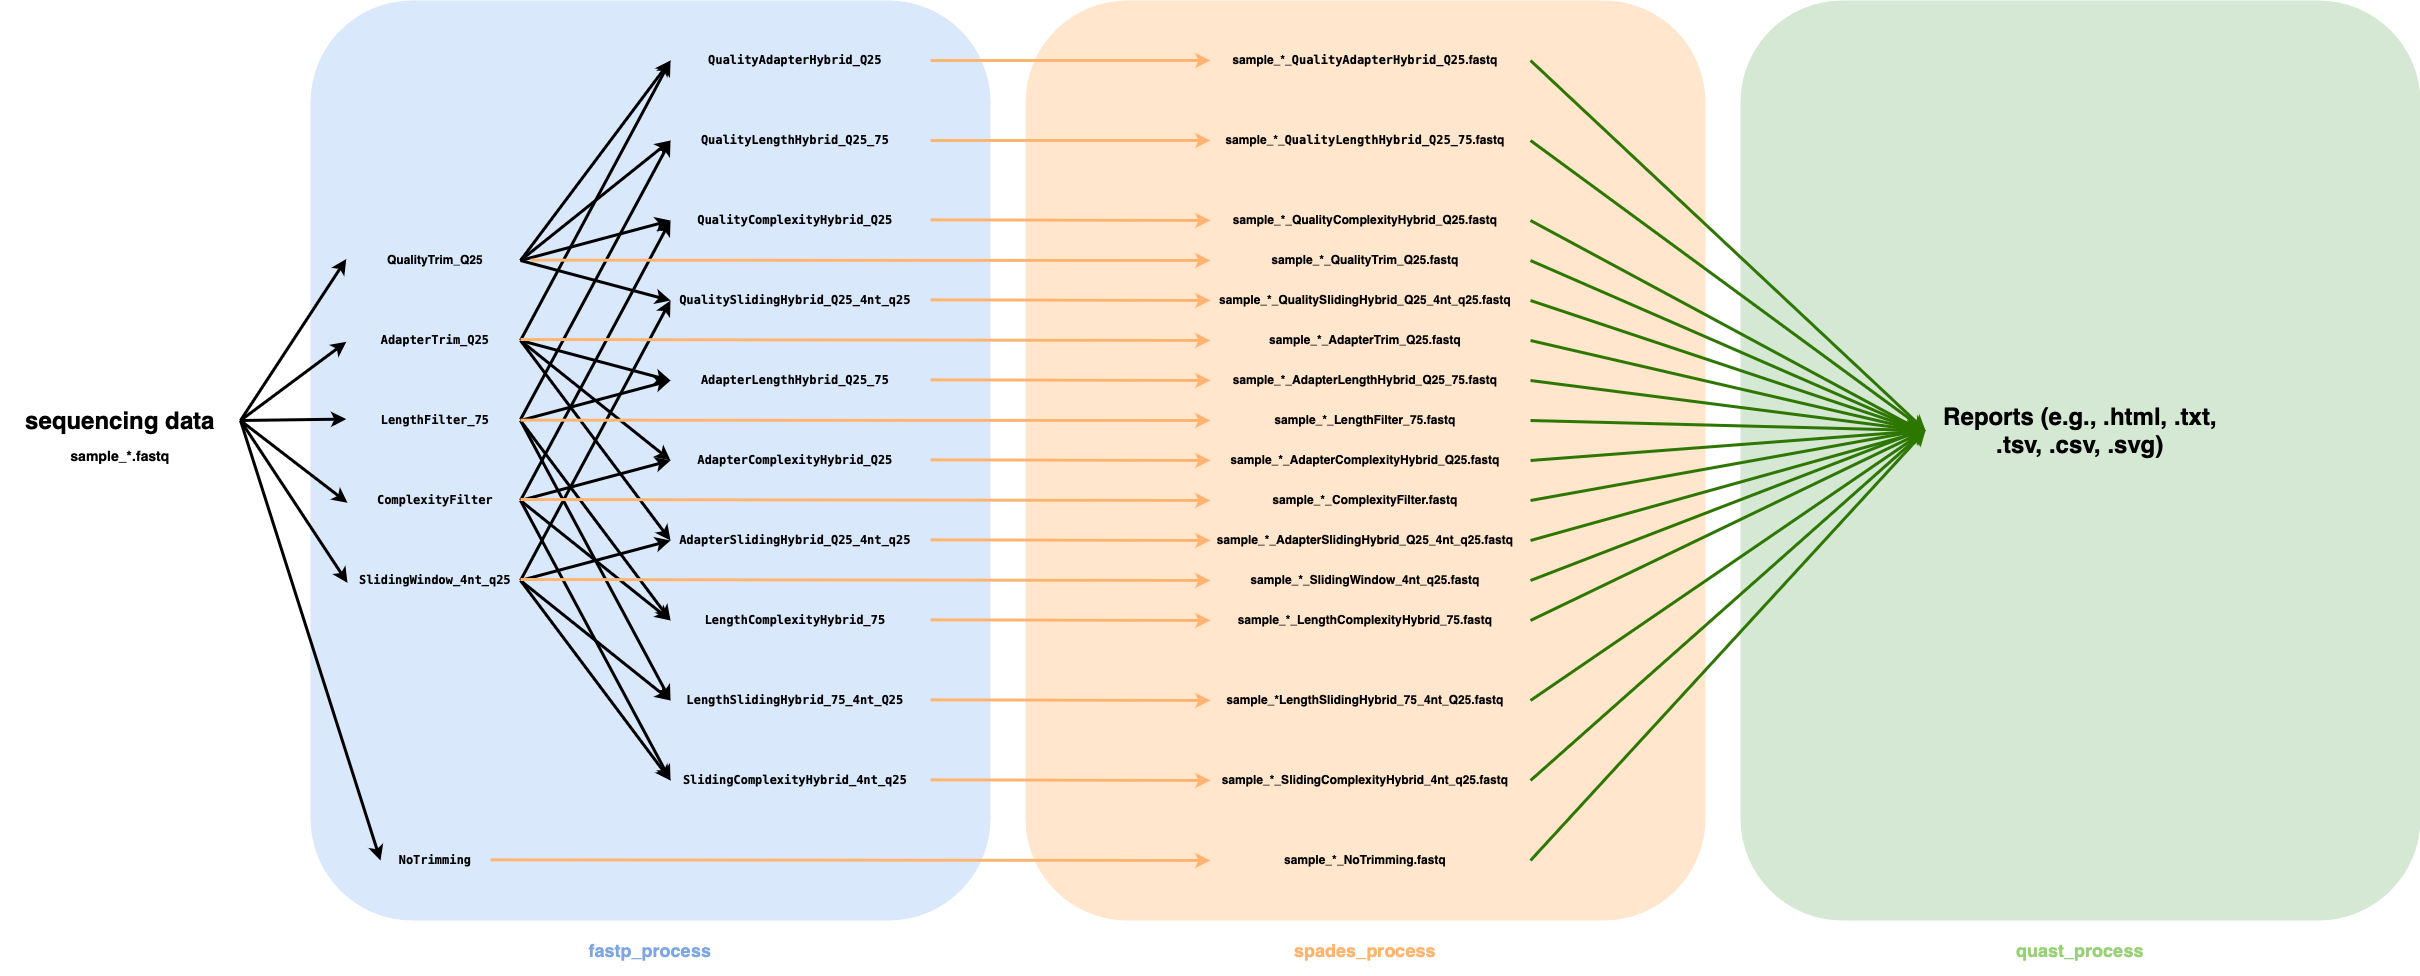
\includegraphics[width=\textwidth]{resources/images/NGS-pipeline.drawio.png}
    \caption{\textbf{Schematic representation of the data flow through the \gls{trimming}, Assembling and Evaluating stages of the software pipeline}. Each \gls{trimming} Method is systematically named to reflect the method and parameters used, ensuring traceability and clarity of the data processing steps.}
    \label{fig:trimming_pipeline}
\end{figure}

The \autoref{fig:trimming_pipeline} illustrates the systematic approach to \gls{trimming}, showcasing the various combinations of methods and their corresponding parameters. This naming consistency allows for each piece of data to be traced through the pipeline, ensuring that the process from initial input to final output, including all intermediate steps, is clear and reproducible.

\paragraph{\gls{trimming} Methods with their Parameters and Expected Outcomes:}

In the initial run of the pipeline, various \gls{trimming} Methods (\autoref{table:basic_trimming_methods} and \autoref{table:hybrid_trimming_methods}) are employed to ensure the highest quality of the sequence data. The table below (\autoref{table:basic_trimming_methods}) summarize the 5 Basic \gls{trimming} Methods, their descriptions, and the expected outcomes upon processing:

\begin{table}[H]
\centering
\begin{tabular}{p{0.2\linewidth} p{0.4\linewidth} p{0.3\linewidth}}
\hline
\textbf{Trimming Method} & \textbf{Description} & \textbf{Expected Result} \\ \hline
NoTrimming & No trimming applied. & Unaltered data \\
QualityTrim\_Q25 & Trims low-quality bases below Q25. & Higher quality \\
AdapterTrim\_Q25 & Removes adapter sequences. & No adapters \\
LengthFilter\_75 & Excludes reads below 75 bases. & Consistent length \\
ComplexityFilter & Filters low complexity sequences. & Reduced complexity \\
SlidingWindow\newline\_4nt\_q25 & Sliding window quality trimming: 4nt window, q25 cutoff & Balanced quality \\
\hline
\end{tabular}
\caption{Basic Trimming Methods in the initial run of the pipeline.}
\label{table:basic_trimming_methods}
\end{table}

Each method is designed to address specific types of artifacts within the sequencing data. The selection of \gls{trimming} Method is crucial to prepare the dataset for accurate assembly and analysis. The most averaged parameters were chosen for each \gls{trimming} Method.

\begin{table}[H]
\centering
\begin{tabular}{l l}
\hline
\textbf{Trimming Method} & \textbf{Expected Result} \\ \hline
QualitySlidingHybrid\_Q25\_4nt\_q25 & Enhanced quality \\
QualityAdapterHybrid\_Q25 & Clean reads \\
LengthComplexityHybrid\_75 & Lengthy, non-repetitive \\
SlidingComplexityHybrid\_4nt\_q25 & Quality, non-repetitive \\
AdapterSlidingHybrid\_Q25\_4nt\_q25 & No adapters, balanced \\
QualityLengthHybrid\_Q25\_75 & High quality, uniform \\
QualityComplexityHybrid\_Q25 & High quality, unique \\
AdapterLengthHybrid\_Q25\_75 & No adapters, consistent \\
AdapterComplexityHybrid\_Q25 & No adapters, unique \\
LengthSlidingHybrid\_75\_4nt\_Q25 & Uniform length, balanced \\
\hline
\end{tabular}
\caption{Hybrid Trimming Methods in the initial run of the pipeline.}
\label{table:hybrid_trimming_methods}
\end{table}

The hybrid \gls{trimming} Methods (\autoref{table:hybrid_trimming_methods}) implemented in the pipeline are the result of combinations without repetitions of the 5 Basic \gls{trimming} Methods. Given 5 Basic \gls{trimming} Methods, the number of unique hybrid combinations that can be created without repeating any single method can be calculated using the formula for combinations without repetition, also known as binomial coefficients. This is mathematically represented as:

\[
C(n, k) = \frac{n!}{k!(n-k)!}
\]

For our case, with \( n = 5 \) basic methods and \( k = 2 \) methods per combination, the formula simplifies to:

\[
C(5, 2) = \frac{5!}{2!(5-2)!} = \frac{5 \times 4}{2 \times 1} = 10
\]

This combinatorial approach yields exactly 10 unique hybrid methods, which are then utilized in the first run of the software pipeline to ensure a comprehensive exploration of \gls{trimming} Effects. That is the reason for choosing exactly 16 \gls{trimming} Methods (10+5+1), including the NoTrimming Method, for the first run of the software pipeline.

\paragraph{The fastp\_process:}

Within the pipeline, the `fastp\_process` is designated to perform Sequence \gls{trimming} and Quality Control. This process is initiated with a unique label and dynamically assigned tags based on \gls{trimming} Parameters and input file names. The input section specifies a tuple consisting of \gls{trimming} Parameters and associated \gls{read} files. The output is similarly structured, producing a tuple that includes the original \gls{trimming} Parameters and paths to the trimmed \gls{fastq} files. It takes \gls{paired-end} \gls{read}s and the \gls{trimming} Parameters as input and generates trimmed sequence files based on the specified parameters. The process dynamically constructs the fastp command based on the \gls{trimming} Method provided, applying the relevant \gls{trimming} Options.

Below is the code to the \textit{fastp\_process}, which is divided into 2 parts (\autoref{lst:fastp} and \autoref{lst:trimming_params_handling}) for ease of reading, in which only essential parts of it are indicated, the rest of the points are commented out for brevity.


\begin{lstlisting}[language=Java, , label={lst:fastp}, caption={Comprehensive Overview of the fastp\_process in the NGS Pipeline.}]
process fastp_process {
    label 'fastp'
    tag "${trimParams}_${reads[0].getName()}"

    input:
        tuple val(trimParams), file(reads)

    output:
        tuple val(trimParams), \
        path("${reads[0].simpleName}_${trimParams}.fastq"), \
        path("${reads[1].simpleName}_${trimParams}.fastq")

    script:
        String trimParamsStr = trimParams.toString().trim()
        def fastpCmd = "fastp --in1 ${reads[0]} --in2 ${reads[1]}"
        String outputFileName1 = "${reads[0].simpleName}_${trimParams}.fastq"
        String outputFileName2 = "${reads[1].simpleName}_${trimParams}.fastq"
        fastpCmd += " --out1 ${outputFileName1} --out2 ${outputFileName2}"
        String htmlReport = "${reads[0].simpleName}_${trimParams}.html"
        String jsonReport = "${reads[0].simpleName}_${trimParams}.json"
        fastpCmd += " --html ${htmlReport} --json ${jsonReport}"

        // Representation of dynamic trimming parameters handling (omitted for brevity)
        // def trimActionMap = [...]
        // trimActionMap.each { key, action -> ... }

        """
        set -euo pipefail
        echo "Trimming parameters: ${trimParams}"
        if [ ${reads.size()} -ne 2 ]; then
            echo "Error: Expected two reads files, but got ${reads.size()}"
            exit 1
        fi
        ${fastpCmd}
        echo "fastp process for ${trimParams}_${reads[0].getName()} completed successfully."
        """
}
\end{lstlisting}

This \autoref{lst:fastp} highlights the input and output file handling, command construction, and application of \gls{trimming} Parameters as part of the \texttt{fastp} command execution within the pipeline. The iterative structure ensures that the appropriate action is taken for each set of \gls{trimming} Parameters. The robustness of the script is evidenced by error handling that checks for the expected pair of \gls{read} files, ensuring data integrity. Upon successful execution, the process concludes with an informative message indicating the completion of the `fastp` operation for the given parameters.

The core of the `fastp\_process` lies in its script section (\autoref{lst:trimming_params_handling}), which constructs the `fastp` command with parameters tailored to the \gls{trimming} Requirements. Here, the \gls{trimming} Parameters are parsed and translated into `fastp` command options. A mapping structure, `trimActionMap`, is defined to convert symbolic \gls{trimming} Names into their respective `fastp` command-line arguments. This approach ensures that each \gls{trimming} Method is applied correctly based on the input data characteristics. 


\begin{lstlisting}[language=Java, , label={lst:trimming_params_handling}, caption={Representation of dynamic trimming parameters handling}]
def parts = trimParamsStr.tokenize('_')

    def trimActionMap = [
    QualityTrim: { String q -> 
      "--qualified_quality_phred ${q.replace('Q', '')}" 
    },
    AdapterTrim: { String q -> 
      "--detect_adapter_for_pe --qualified_quality_phred " +
      "${q.replace('Q', '')}" 
    },
    
    // The rest of the trimming methods that are omitted for brevity
    
    NoTrimming: { _ -> 
      "--disable_adapter_trimming --disable_quality_filtering " +
      "--disable_length_filtering" 
    }
    ]

    trimActionMap.each { key, action ->
    if (trimParamsStr.startsWith(key)) {
        fastpCmd += " " + action(parts.drop(1))
        return
      }
    }
\end{lstlisting}

For example, based on the \gls{trimming} Method "QualityTrim\_Q25" a fastp command will be dynamically created (\autoref{lst:trimming_params_handling}) with the parameter "-qualified\_quality\_phred" and the quality value 25 will be automatically added (the numbers are also dynamically set) means phred quality >=Q25 is qualified. In this example a quality value of 25 corresponds to an error probability of 1 in 100 (i.e., 99\% accuracy), which is a fairly high threshold for many bioinformatics and genomics applications.


Different combinations (\autoref{tab:phred_scores}) of \gls{sequencing} quality parameters (Phred-Score Q) such as Q15, Q20, Q25, and Q30 are presented within this work. These parameters are used to provide varying degrees of rigor in \gls{trimming} \gls{read}s, allowing the data cleaning process to be customized for specific study purposes.

\begin{table}[ht]
\centering
\begin{tabular}{cc}
\hline
\textbf{Phred-Score Q} & \textbf{Accurancy (\%)} \\
\hline
Q15 & 99.97\% \\
Q20 & 99.99\% \\
Q25 & 99.999\% \\
Q30 & 99.9999\% \\
\end{tabular}
\caption{Correlation between Phred-Score Q and percentage accuracy.}
\label{tab:phred_scores}
\end{table}




\subsection{SPAdes for Genome Assembly}
For the \gls{assembly} stage, \textit{SPAdes} (St. Petersburg genome assembler) was chosen for its versatility and effectiveness in assembling high-quality \gls{genome}s from \gls{ngs} data coming from the preceding \texttt{fastp\_process} (\autoref{lst:fastp}). In our project, \textit{SPAdes} was employed to construct high-quality genomic assemblies from the preprocessed \gls{read}s. The assembler's advanced algorithms enable the reconstruction of genomic sequences with high accuracy, making it an indispensable tool for our software pipeline.

\paragraph{The spades\_process:}

The \autoref{lst:spades}represents the \texttt{spades\_process} within the Nextflow pipeline, aimed at conducting \gls{assembly} utilizing the SPAdes Software. This process is integral to transforming Sequencing \gls{read}s into Assembled \gls{genome}s, a crucial step in understanding the genomic architecture of the organism under study.

\begin{lstlisting}[language=Java, label={lst:spades}, caption={SPAdes genome assembly process in Nextflow.}]
process spades_process {
  label 'spades'
  tag "${trimParams}"

  input:
    tuple val(trimParams), path(read1), path(read2)
    
  output:
    path "scaffolds_${trimParams}.fasta"

  cpus 4
  memory '8 GB'

  script:
    """
    set -euo pipefail
    echo "Read1: ${read1}"
    echo "Read2: ${read2}"
    echo "Starting SPAdes genome assembly for ${trimParams}..."
    spades.py --isolate -1 ${read1} -2 ${read2} -o output_${trimParams}
    mv output_${trimParams}/scaffolds.fasta scaffolds_${trimParams}.fasta
    echo "SPAdes genome assembly for ${trimParams} completed successfully."
    """
}
\end{lstlisting}

\textbf{Key Components of the \autoref{lst:spades}:}

\begin{itemize}
    \item \textbf{Label and Tag:} The process is labeled 'spades' and tagged with \gls{trimming} Parameters, facilitating resource allocation and identification of the process's tasks.
    \item \textbf{Input:} Accepts a tuple comprising \gls{trimming} Parameters and paths to paired-end \gls{read} files, signifying the raw data for \gls{assembly}.
    \item \textbf{Output:} Produces a FASTA file named after the \gls{trimming} Parameters, containing the assembled \gls{scaffold}s, which are the result of the SPAdes assembly process.
    \item \textbf{Resources:} Allocated with 4 CPUs and 8 GB of memory, ensuring sufficient computational resources for the assembly task. (This parameter can be adjusted to suit the needs and power of the computer individually. This demonstrates the parameters used in this study.)
    \item \textbf{Script:} Executes the SPAdes command with the provided \gls{read}s, outputting the \gls{assembly} into a designated folder, subsequently moving the \gls{scaffold}s file to a specified path. The use of \texttt{set -euo pipefail} parameter ensures that the script will stop if errors occur, which increases the reliability of the process execution.
\end{itemize}

This process exemplifies a critical step (\autoref{lst:spades}) in the software pipeline, converting Trimmed Sequencing \gls{read}s into a coherent genomic structure, thereby enabling further genomic analyses.


\subsection{QUAST for Quality Assessment}
Upon completion of the \gls{assembly}, \textit{QUAST} (Quality Assessment Tool for Genome Assemblies) was utilized to evaluate the quality of the assembled sequences. \textit{QUAST} provides comprehensive Quality \gls{metrics}, including contiguity, coverage, and correctness of the assemblies. By applying \textit{QUAST}, we were able to assess the assembly quality in a quantitative manner, allowing for the identification and correction of potential errors in the \autoref{lst:spades} Assembled \gls{genome}s. This quality assessment step is crucial for ensuring that the final genomic sequences are accurate and suitable for downstream analyses.

\paragraph{The quast\_process:}

described below (\autoref{lst:quast}), is an important component of the software pipeline designed to evaluate genomic assemblies derived from the previous \texttt{spades\_process} using QUAST. This process facilitates \gls{assembly} Quality Assessment by providing critical insight into the integrity and completeness of Assembled \gls{genome}s. This creates reports on each \gls{genome} collected here, which we then analyze. Different file extensions are available to choose from, e.g. TSV, which we use in further analysis.

\begin{lstlisting}[language=Java, label={lst:quast}, caption={QUAST quality assessment process in Nextflow.}]
process quast_process {

  input:
    path genomes

  output:
    path "reports"

  script:
    """
    mkdir -p reports
    set -euo pipefail
    for genome in ${genomes}
    do
      genome_name=\$(basename \$genome .fasta)
      echo "Starting QUAST quality assessment for \$genome_name..."
      quast.py -o reports/output_\${genome_name} \${genome}
      mv reports/output_\${genome_name}/report.html \
        reports/report_\${genome_name}.html
      echo "QUAST quality assessment for \$genome_name completed."
    done
    """
}
\end{lstlisting}

\textbf{Key Elements of the \autoref{lst:quast}:}

\begin{itemize}
    \item \textbf{Input:} It accepts a path to \gls{genome} Assemblies, serving as the input for the quality assessment procedure.
    \item \textbf{Output:} Generates a directory named "reports" which will contain HTML reports for each Analyzed \gls{genome}, summarizing the quality assessment results.
    \item \textbf{Script:} This segment of the process encapsulates the commands for executing QUAST on each \gls{assembly}, highlighting the iterative approach to generate comprehensive quality reports. The use of a loop to process multiple \gls{genome}s and the subsequent organization of reports demonstrate the process's capability to handle batch assessments, making it a scalable solution for quality analysis.
\end{itemize}

Overall, \texttt{quast\_process} (\autoref{lst:quast}) represents an important step towards ensuring the reliability of genomic assemblies by offering a systematic approach to quality control in genomic research.













\section{Pipeline Implementation}

\subsection{Initial Setup in Nextflow}

The provided \autoref{lst:initial} is a crucial component of a Nextflow pipeline designed for processing \gls{ngs} data. This segment outlines the initial setup for data preprocessing, specifically focusing on the diversity of \gls{trimming} Methods applied prior to \gls{assembly} and Quality Assessment.

\begin{lstlisting}[language=Java, label={lst:initial}, caption={Initial setup and trimming strategy definition in Nextflow.}]
// Define input and output directory parameters
params.input_dir = 'raw_data'

// Define a list of different trimming combinations for sequence processing
def trimmingCombinations = [
  "QualityTrim_Q25",
  "AdapterTrim_Q25",
  "LengthFilter_75",
  "ComplexityFilter",
  "SlidingWindow_4nt_q25",
  "QualitySlidingHybrid_Q25_4nt_q25", // QualityTrim_Q25 + SlidingWindow_4nt_q25
  // Other trimming combinations
  "NoTrimming"
]

/* Create a channel with trimming combinations 
  and pair them with file pairs from the input directory
*/
Channel
  .from(trimmingCombinations)
  .combine(Channel.fromFilePairs("${params.input_dir}/*_{1,2}.fastq"))
  .map { trimParams, sampleId, files -> 
    println("Trim Params: ${trimParams}, Files: ${files}") 
    tuple(trimParams, files) 
  }
  .set { trimmingChannel }

\end{lstlisting}

\textbf{Key Elements of the \autoref{lst:initial}:}

\begin{itemize}
    \item \textbf{Parameter Definition:} The script begins by setting the input directory parameter, which specifies the location of raw \gls{sequencing} Data.
    \item \textbf{Trimming Combinations:} A comprehensive list of \gls{trimming} Methods is defined, encompassing a variety of approaches to clean and prepare the data for subsequent analysis stages. This list demonstrates the pipeline's flexibility in handling different data quality concerns.
    \item \textbf{Channel Creation:} The script dynamically creates a channel that pairs \gls{trimming} Combinations with \gls{sequencing} file pairs, facilitating the parallel processing of data with various \gls{trimming} Settings.
\end{itemize}

This script exemplifies a structured and efficient approach to \gls{ngs} data preprocessing, showcasing Nextflow's capability to orchestrate complex bioinformatics workflows with ease.


\subsection{Workflow Execution}

\begin{lstlisting}[language=Java, label={lst:workflow}, caption={The workflow section.}]
workflow {
  fastp_process(trimmingChannel)
    .groupTuple()
    .set { fastpCollectChannel }

  spades_process(fastpCollectChannel)
    .collect()
    .set { quastInputChannel }

  quast_process(quastInputChannel)
}
\end{lstlisting}

The workflow section (\autoref{lst:workflow}) illustrates the sequential execution of processes: `fastp\_process` for \gls{read} \gls{trimming}, `spades\_process` for \gls{assembly}, and `quast\_process` for Assembly Quality Assessment. This structure underscores the pipeline's cohesive approach to \gls{ngs} data analysis.

\subsection{Trimming Strategies}


\gls{trimming} Strategies refer to a predetermined list of \gls{trimming} Combinations employed during individual runs of our software pipeline to identify the optimal approach for data preprocessing. These strategies are crucial for enhancing data quality by removing low-quality bases, adapter sequences, and other undesirable elements from raw \gls{sequencing} Data. The selection of a specific \gls{trimming} Strategy is detailed in the subsequent section titled ``Results.'' Within the context of this study, three distinct \gls{trimming} Strategies were implemented, corresponding to three separate executions of the pipeline. Each strategy was designed to explore a range of \gls{trimming} Parameters and their impact on the subsequent analysis, thereby facilitating an informed decision on the most effective preprocessing steps for our dataset.


Three \gls{trimming} Strategies (\autoref{tab:comprehensive_trimming_strategies}) were devised to evaluate the performance of various \gls{trimming} Parameters systematically. The strategies encompass a broad spectrum of \gls{trimming} Options, including quality threshold adjustments, adapter trimming, length filtering, and complexity filtering among others. The intention behind these strategies is to ascertain the combination that yields the highest quality of Processed \gls{read}s, which is pivotal for the reliability of downstream analyses such as \gls{assembly} or variant calling. The results section will elucidate the outcomes of employing each \gls{trimming} Strategy on the dataset, presenting a comparative analysis of their efficacy based on metrics such as data retention, quality improvement, and impact on downstream analyses. 

\begin{table}[h!]
\centering
\caption{Comprehensive Trimming Strategies Employed Across Three Pipeline Runs}
\label{tab:comprehensive_trimming_strategies}
\resizebox{\textwidth}{!}{%
\begin{tabular}{|l|l|l|}
\hline
\textbf{The 1st Trimming Strategy}                 & \textbf{The 2nd Trimming Strategy}            & \textbf{The 3rd Trimming Strategy}           \\ \hline
QualityTrim\_Q25                            & SlidingWindow\_4nt\_q15                 & SlidingWindow\_3nt\_q30               \\
AdapterTrim\_Q25                            & SlidingWindow\_4nt\_q20                 & SlidingWindow\_4nt\_q30               \\
LengthFilter\_75                            & SlidingWindow\_4nt\_q25                 & SlidingWindow\_4nt\_q29               \\
ComplexityFilter                            & SlidingWindow\_4nt\_q30                 & SlidingWindow\_5nt\_q30               \\
SlidingWindow\_4nt\_q25                     & SlidingWindow\_7nt\_q15                 & LengthFilter\_30                      \\
QualitySlidingHybrid\_Q25\_4nt\_q25         & SlidingWindow\_7nt\_q20                 & LengthFilter\_35                      \\
QualityAdapterHybrid\_Q25                   & SlidingWindow\_7nt\_q25                 & LengthFilter\_40                      \\
LengthComplexityHybrid\_75                  & SlidingWindow\_7nt\_q30                 & LengthFilter\_45                      \\
SlidingComplexityHybrid\_4nt\_q25           & SlidingWindow\_10nt\_q15                & LengthFilter\_50                      \\
AdapterSlidingHybrid\_Q25\_4nt\_q25         & SlidingWindow\_10nt\_q20                & LengthFilter\_55                      \\
QualityLengthHybrid\_Q25\_75                & SlidingWindow\_10nt\_q25                &                                      \\
QualityComplexityHybrid\_Q25               & SlidingWindow\_10nt\_q30                &                                      \\
AdapterLengthHybrid\_Q25\_75                & SlidingWindow\_20nt\_q15                &                                      \\
AdapterComplexityHybrid\_Q25               & SlidingWindow\_20nt\_q20                &                                      \\
LengthSlidingHybrid\_75\_4nt\_Q25           & SlidingWindow\_20nt\_q25                &                                      \\
NoTrimming                                  & SlidingWindow\_20nt\_q30                &                                      \\
                                            & LengthFilter\_50                        &                                      \\
                                            & LengthFilter\_75                        &                                      \\
                                            & LengthFilter\_100                       &                                      \\
                                            & LengthFilter\_150                       &                                      \\
                                            & LengthFilter\_200                       &                                      \\
                                            & LengthFilter\_250                       &                                      \\ \hline
\end{tabular}%
}
\end{table}


Therefore, \textbf{48} \gls{genome}s with different Data \gls{trimming} Parameters (\autoref{tab:comprehensive_trimming_strategies}) were assembled and analyzed as part of this work using this pipeline. In total, it took tens of hours of computing time and dozens of gigabytes of memory.







